%% Hustle for Cash: Evidence from Nigeria's Naira Crunch
%% Main file — compile with pdflatex
%% All table notes via threeparttable; figure notes via floatrow
%% Never cut a note off the bottom of a float.

\documentclass[12pt]{article}

% ── Typography and layout ──────────────────────────────────────────────────────
\usepackage[margin=1in]{geometry}
\usepackage{setspace}
\onehalfspacing
\usepackage[T1]{fontenc}
\usepackage[utf8]{inputenc}
\usepackage{microtype}
\usepackage{lmodern}

% ── Maths ─────────────────────────────────────────────────────────────────────
\usepackage{amsmath,amssymb,amsthm}

% ── Tables ────────────────────────────────────────────────────────────────────
\usepackage{booktabs}
\usepackage{threeparttable}   % keeps notes with their table, never orphaned
\usepackage{multirow}
\usepackage{array}
\usepackage{dcolumn}          % decimal-aligned columns
\usepackage{siunitx}
\sisetup{
  table-format          = -2.3,
  table-number-alignment = center,
  group-separator       = {,}
}
\usepackage{tabularx}

% ── Figures ───────────────────────────────────────────────────────────────────
\usepackage{graphicx}
\usepackage{floatrow}         % \floatfoot keeps notes inside figure floats
\floatsetup[figure]{capposition=bottom}
\floatsetup[table]{style=plaintop}
\usepackage{subcaption}
\usepackage{caption}
\captionsetup{
  font=small,
  labelfont=bf,
  labelsep=period,
  skip=6pt
}

% ── Float placement ───────────────────────────────────────────────────────────
\usepackage{float}
\usepackage{placeins}         % \FloatBarrier

% ── Hyperlinks ────────────────────────────────────────────────────────────────
\usepackage[
  colorlinks = true,
  linkcolor  = black,
  citecolor  = black,
  urlcolor   = blue
]{hyperref}

% ── Bibliography ──────────────────────────────────────────────────────────────
\usepackage{natbib}
\bibliographystyle{plainnat}   % author-year citations via natbib
\setcitestyle{authoryear,open={(},close={)}}

% ── Miscellaneous ─────────────────────────────────────────────────────────────
\usepackage{enumitem}
\usepackage{xcolor}
\usepackage{pdflscape}        % landscape pages for wide tables
\usepackage{afterpage}
\usepackage{appendix}

% ── Theorem environments ──────────────────────────────────────────────────────
\newtheorem{proposition}{Proposition}
\newtheorem{lemma}{Lemma}
\newtheorem{corollary}{Corollary}
\theoremstyle{remark}
\newtheorem{remark}{Remark}

% ── Custom commands ───────────────────────────────────────────────────────────
\newcommand{\std}[1]{\ensuremath{(#1)}}          % std errors below coeff
\newcommand{\placeholder}[1]{\textcolor{red}{[#1]}}  % fill-in markers
\newcommand{\VIIRS}{\textsc{viirs}}
\newcommand{\NLPS}{\textsc{nlps}}
\newcommand{\WBES}{\textsc{wbes}}
\newcommand{\NTL}{\textsc{ntl}}
\newcommand{\CBN}{\textsc{cbn}}
\newcommand{\naira}{%
  \mbox{N\kern-.55em\raisebox{.35ex}{\rule{.5em}{.4pt}}\kern.05em}}

% ─────────────────────────────────────────────────────────────────────────────

\begin{document}

% ── Title page ────────────────────────────────────────────────────────────────
\title{%
  Hustle for Cash:\\
  Evidence from Nigeria's Naira Crunch%
}

\author{%
  Abiodun Adetokunbo%
  \thanks{%
    Augustine University, Lagos, Nigeria.
    E-mail: \href{mailto:abiodun.adetokunbo@augustineuniversity.edu.ng}%
      {abiodun.adetokunbo@augustineuniversity.edu.ng}.%
  }%
}


\date{\today}
\maketitle
\thispagestyle{empty}

% ── Abstract ──────────────────────────────────────────────────────────────────
\begin{abstract}
\noindent
When Nigeria's central bank abruptly withdrew currency in late 2022 and capped
cash withdrawals, the resulting shortage, the \emph{naira crunch}, created
a sharp, unanticipated cash supply shock. This paper exploits cross-state
variation in pre-shock digital payment adoption, measured eleven days before
the policy announcement, to estimate the real costs of the crunch and the
insulating role of financial infrastructure. Using enterprise modules from the
Nigeria Living Standards Phone Survey (1,842 household enterprises across three
rounds), with the parallel-trends assumption validated through a 45-month
pre-shock nighttime-light panel covering all 774 Nigerian local government
areas, enterprises in states one standard deviation above the pre-shock fintech
mean were 1.7 percentage points more likely to remain in operation at peak
crunch and 7.7 percentage points more likely to survive fourteen months later.
Employment effects are also large: 0.29 additional enterprise workers per
standard deviation of fintech at peak crunch.
Effects are concentrated in rural and small enterprises. The results identify
digital financial infrastructure as a macroeconomic stabiliser against cash
supply disruptions, with implications for central bank currency operations in
low-income economies.

\medskip
\noindent
\textbf{JEL codes:} E41, E52, G23, O16, O55

\noindent
\textbf{Keywords:} cash supply shock, digital payments, fintech, nighttime
lights, Nigeria, demonetisation
\end{abstract}

\clearpage
\setcounter{page}{1}

% ── Sections ──────────────────────────────────────────────────────────────────
%% Section 1: Introduction

\section{Introduction}
\label{sec:intro}

In late October 2022, Nigeria's central bank announced the withdrawal and
redesign of its currency notes, together with strict daily caps on cash
withdrawals. By January 2023, a rolling shortage of the replacement notes had
produced hour-long queues outside commercial banks, paralysed point-of-sale
terminals, and darkened markets where almost every transaction had always
settled in cash. Prices for essential goods spiked and some small enterprises closed
their doors. In February 2023 the Supreme Court ordered the old notes to remain
legal tender, and the central bank progressively released more new currency
over the following months. The episode, the \emph{naira crunch}, lasted
approximately six months before cash supply normalised.

The crunch was an abrupt, policy-induced cash supply shock where the stock of
physical currency available for transactions fell sharply while the demand for
cash-settled transactions did not. Its severity, however, varied substantially
across Nigeria's thirty-six states and the Federal Capital Territory
(\textsc{fct}), for a reason not immediately obvious at
the time as some states had higher pre-shock adoption of digital
payment technology. In those states, enterprises and households could substitute
to mobile money wallets, USSD bank transfers, and fintech applications when
ATMs ran dry. In states where most transactions still settled exclusively in
cash, limited substitute existed.

This paper exploits that cross-sectional heterogeneity to estimate the real
costs of a cash supply shock and the extent to which digital financial
infrastructure acts as a buffer. The identification relies on three features
of the episode. First, the \CBN{} announcement on October~26, 2022 was
genuinely unanticipated, making the pre-shock distribution of fintech
adoption a predetermined variable uncontaminated by anticipation of the shock.
Second, that distribution is measured using the Nigeria Living Standards
Phone Survey (\NLPS) Round~6 which was conducted on October~15, 2022, eleven days
before the announcement, providing a state-level index of digital payment
penetration constructed from four digital-payment service categories.\footnote{%
  The index uses four digital-payment categories: mobile money, commercial
  bank accounts, mobile and \textsc{ussd} banking, and mobile banking
  applications. Four further categories (pension/insurance, securities,
  microfinance, and credit cards) are excluded because their penetration is
  below 4\% in all states and they do not constitute a meaningful cash
  substitute during the crunch; see Appendix~Table~\ref{atab:alt_treatment}
  for robustness to alternative index definitions.
  Section~\ref{sec:data} details the construction.}
Third, the parallel-trends assumption is validated using monthly composites of
nighttime-light radiance from the \textsc{nasa} \VIIRS{} Black Marble satellite
product for all 774 Nigerian local government areas (January~2019 to
September~2022), providing 45 consecutive pre-shock months over which
high- and low-fintech states can be shown to have followed statistically
identical trajectories prior to the crunch. Section~\ref{sec:design} details
the identification strategy and pre-trend validation.

The primary evidence comes from firm-level data.and the main findings are as follows.
Enterprises in states one standard deviation above the pre-shock fintech
mean were 1.7 percentage points more likely to remain in operation at the
February 2023 peak crunch and 7.7 percentage points more likely
to remain in operation fourteen months later in April 2024.
Employment was also significantly insulated as high-fintech states had
0.29 more enterprise workers during the peak crunch. 
Effects are concentrated in rural firms and small enterprises below-median
size, the units most dependent on daily cash flow.

These results contribute to three literatures. First, they extend
\citet{chodorow2020cash} to the mobile-money studies. \citet{chodorow2020cash} shows that
Indian districts with fewer bank branches lost more economic activity during
the 2016 demonetisation; the relevant margin in Sub-Saharan Africa is not bank
branches, but digital payment technology.
This paper identifies a \emph{digital payment substitution channel} that the
India paper's design, which relies on bank-deposit variation, cannot isolate.
The magnitude of the enterprise-survival estimates implies that closing the
fintech adoption gap between the 10th- and 90th-percentile Nigerian states
would have reduced firm exit at the peak crunch by approximately 5 percentage
points, a substantial share of the 16-percentage-point decline in enterprise
activity observed between Round~5 and Round~7.

Second, this paper provides evidence for a digital-payment substitution mechanism 
emphasized in the mobile-money literature. By enabling transactions and transfers to be 
executed without physical currency, digital payment technologies reduce reliance on 
cash and may attenuate the effects of cash-supply disruptions \citep{jack2014risk}. 
The present study quantifies the extent of this insulation 
in LMICs using plausibly exogenous pre-determined variation in fintech adoption. 


Third, the analysis contributes to the emerging methodological literature on
identifying monetary transmission in data-sparse economies by leveraging alternative proxies 
for economic activity 
\citep[see][]{henderson2012measuring,donaldson2016view}. High-frequency satellite
imagery combined with granular phone survey data can recover real monetary
transmission at subnational resolution where the formal national accounts
provide limited quarterly or monthly benchmarks. The satellite--survey combination
is directly replicable for other African central bank episodes.

Section~\ref{sec:context} describes the naira crunch and Nigeria's payment
landscape. Section~\ref{sec:literature} surveys the related literature.
Section~\ref{sec:theory} presents the theoretical framework.
Section~\ref{sec:data} introduces the data. Section~\ref{sec:design}
presents the research design and validates the identifying assumption using
the 45-month \NTL{} pre-trend window. Section~\ref{sec:results_micro} reports
the firm-level results. Section~\ref{sec:longrun} examines longer-run effects
using the 2025 World Bank Enterprise Survey and the April 2024 \NLPS{} round.
Section~\ref{sec:conclusion} concludes with policy implications.

%% Section 2: Institutional Context

\section{The Naira Crunch: Institutional Context}
\label{sec:context}

\subsection{The Policy Shock}

On October~26, 2022, the Central Bank of Nigeria (\CBN) announced the
redesign of its three highest-denomination banknotes (₦200, ₦500, and
₦1,000) and set a January~31, 2023 deadline for old notes to be
deposited and replaced \citep{cbn2022circular}. Daily ATM withdrawals
were capped at ₦20,000 (approximately \$43 at the prevailing
rate) and over-the-counter withdrawals at ₦100,000 per week.
The stated rationale was to combat counterfeiting, reduce the volume
of currency held outside the banking system, and accelerate the
adoption of digital payments in support of the \CBN's broader
cashless-economy agenda.

The roll-out of new notes proved severely inadequate to demand. By
mid-January 2023, queues outside commercial banks and ATMs stretched
for hours across major Nigerian cities. Reports from the field and
media documentation consistently describe near-total unavailability
of new notes in rural areas, with POS machines dysfunctional and
markets at a standstill.\footnote{%
  The \emph{NBS Enterprise Telephone Survey}, \emph{SBM Intelligence}
  rapid surveys, and contemporaneous New Agency of Nigeria \emph{NAN} wire reports provide
  granular documentation. These sources are not used for
  identification; they motivate the timing of the shock indicators.}
The naira crunch was by this point a genuine constraint on economic
activity, not merely an inconvenience.

In February 2023 Supreme Court of Nigeria ruled that old notes must
remain legal tender until December 2023, providing partial relief.
Concurrently, the \CBN{} accelerated distribution of new currency.
By mid-2023 most commercial channels had normalised, though
\NLPS{} survey evidence (Round~11, April 2024) and the 2025 \WBES{}
both indicate persistent behavioural shifts in payment habits.

Table~\ref{tab:shock_timeline} summarises the shock timeline.

\begin{table}[H]
\begin{threeparttable}
\caption{Naira Crunch: Policy Timeline}
\label{tab:shock_timeline}
\small
\begin{tabularx}{\textwidth}{lX}
\toprule
\textbf{Date} & \textbf{Event} \\
\midrule
October 26, 2022
  & \CBN{} announces naira redesign; caps daily ATM withdrawals
    at ₦20,000; sets January 31 deadline for old notes. \\[4pt]
November--December 2022
  & Transition period: old notes recalled, new notes printed but
    distribution severely below demand. Early shortages in
    smaller cities and rural areas. \\[4pt]
January--February 2023
  & \emph{Peak crunch}: near-complete ATM dry-outs in many states;
    hour-long bank queues; POS network failures; informal market
    disruption. \\[4pt]
February 8, 2023
  & Supreme Court orders old notes remain legal tender;
    \CBN{} given three weeks to increase note supply. \\[4pt]
March--June 2023
  & Gradual recovery as new note circulation increases;
    cash availability improves progressively by state. \\[4pt]
July 2023 onward
  & Post-crunch: cash supply normalised in most states;
    some permanent shift toward digital payment habits
    documented in subsequent surveys. \\
\bottomrule
\end{tabularx}
\begin{tablenotes}
\footnotesize
\item \textit{Notes:} Timeline constructed from \CBN{} official
  circulars, Supreme Court records, and National Bureau of Statistics
  rapid-survey documentation. Shock indicator periods follow this
  timeline exactly; see Section~\ref{sec:design} for period definitions.
\end{tablenotes}
\end{threeparttable}
\end{table}

\subsection{Nigeria's Payment Landscape}
\label{sub:payment_landscape}

Understanding why fintech adoption creates differential exposure
requires appreciating Nigeria's payment infrastructure at the time of
the shock. According to the 2021 \emph{Global Findex}, approximately
45 percent of Nigerian adults held a formal bank account, well below
South Africa (85\%).
Bank branch density is heavily concentrated in Lagos, Abuja, Port
Harcourt, and Kano; many northern and rural states have fewer than
two commercial bank branches per 100,000 inhabitants \citep{IMF2022FAS}.

Against this low-baseline context, fintech adoption expanded rapidly
between 2018 and 2022. Three developments are particularly relevant.
First, mobile money operators (notably OPay and PalmPay) scaled
their agent networks aggressively, reaching peri-urban and rural
areas bypassed by traditional banking. Second, the \CBN{}'s
mandatory tier-1 Know-Your-Customer (\textsc{kyc}) relaxation in 2018
lowered barriers to opening mobile wallets. Third, \textsc{ussd} banking
(dialling a short code to transact without internet) penetrated widely
through the mobile network operator infrastructure.

A concern is whether these \CBN{}-directed policies render fintech
adoption endogenous to the 2022 crunch that if states that responded most to
the 2018 \textsc{kyc} relaxation were also anticipating a cashless policy,
the pre-shock fintech index might proxy for policy expectations rather than
exogenous infrastructure variation. Three features of the episode address
this concern. First, the specific form of the 2022 shock, a forced currency
redesign combined with withdrawal caps, was not a predictable consequence of
the 2018 \textsc{kyc} relaxation; the two episodes are legally and operationally
distinct, separated by four years. Second, the \NLPS{} Round~6 financial
service module, conducted 11~days before the announcement, directly records
\emph{realised} adoption, not plans or expectations. Also, the comparison of
Round~6 to Round~7 (February 2023) shows significant changes in financial
service usage, confirming agents had not positioned in advance. Third,
cross-state variation in fintech take-up shows differential adoption of
mobile infrastructure, driven by geography, agent-network rollout costs, and
pre-existing mobile penetration, rather than differential anticipation of
currency policy, as the geographic analysis in Section~\ref{sub:iv} shows.

By October 2022, the \NLPS{} Round~6 financial services module
(conducted 11 days before the \CBN{} announcement) recorded the
following state-level averages. 14.7 percent of households held a
commercial bank account; 86.2 percent had used mobile phone or
\textsc{ussd} banking; 5.9 percent held a mobile money account;
and 5.1 percent used a mobile banking application. The composite
fintech index, the simple average of the four digital-payment
categories, ranged from 19.8\,\% (Oyo) to 40.5\,\% (Taraba) across
states, providing the cross-sectional variation the identification exploits.

States with low fintech penetration are not simply poorer.
Appendix~Table~\ref{atab:fintech_correlates} shows that the
state-level fintech index is uncorrelated with pre-2022
nighttime light intensity ($r = -0.19$) and with pre-trend \NTL{}
growth ($r = 0.10$), supporting the parallel-trends assumption
formalised in Section~\ref{sec:design}.

%% Section 3: Related Literature

\section{Related Literature}
\label{sec:literature}

This paper contributes to four bodies of work as it relates to the economic effects of
cash supply shocks, the role of digital payment technology in developing
economies, the theory of money and payment systems, and the use of satellite
nighttime lights as a high-frequency economic indicator.

\subsection{Cash Supply Shocks and Currency Policy}

The empirical literature on cash supply shocks is anchored by India's
November 2016 demonetisation, when the government abruptly invalidated
86 percent of the currency in circulation. \citet{chodorow2020cash} exploit
geographic distribution of demonetized versus newly printed 
bank notes across India's districts, and find that districts with fewer
bank branches and higher cash reliance experienced significantly larger
declines in economic activity, measured by nighttime lights and formal
employment. In sub-Saharan Africa specifically in Nigeria, a relevant margin of 
financial access is  digital
payment technology that operates independently of physical branch
infrastructure. This motivates the focus of this study on a fintech-based
treatment variable and isolates a \emph{digital payment substitution channel}.

\citet{lahiri2020demonetization} provides a complementary macroeconomic
accounting of the 2016 episode, documenting that the GDP cost was concentrated
in the informal sector and in the months immediately following the shock.
\citet{rogoff2015costs} argues that the aggregate macroeconomic benefits of
reducing paper currency use are substantial.  Evidence from this current study points to an
important asymmetry where reducing cash dependence through digital payment adoption is
welfare-improving, but an abrupt withdrawal of currency without sufficient
digital infrastructure to substitute imposes large real costs concentrated in
the least financially included segments of the economy.

\subsection{Digital Payments and Financial Inclusion}

The literature has established the welfare effects of mobile money and digital
payment technology in low-income settings. \citet{jack2014risk} provide the
foundational causal evidence from Kenya's M-Pesa system, showing that mobile
money enables households to share risk more effectively and smooth consumption
against income shocks. \citet{suri2016mobile} extend this to long-run poverty
outcomes, finding that mobile money adoption increased per-capita consumption
and reduced poverty, with larger effects for female-headed households.
\citet{MbitiWeil2016} finds that increased use of M-Pesa lowers the propensity to use informal savings 
mechanisms and raises the likelihood of being banked.

In West Africa, \citet{aker2016payment} evaluate a mobile-money
cash transfer programme in Niger and find significant reductions in transaction
costs and improvements in household welfare relative to traditional payment
channels. These studies establish that digital payment access provides direct
welfare benefits through risk-sharing and consumption smoothing. The
contribution of this study is to identify digital payment
infrastructure as a stabiliser that insulates the real economy
from disruptions in the supply of physical currency. This channel operates at
the state level rather than the household level and is distinct from the
individual-level welfare gains that had been shown in earlier studies.

Financial inclusion literature, \citet{beck2007finance},
\citet{allen2016foundations}, \citet{burgess2005rural}, had shown  that access
to formal financial services promotes household welfare and firm productivity
through credit access, risk management, and reduced transaction costs. The
naira crunch episode allows us to estimate the value of financial
infrastructure through its performance under stress, when infrastructure 
serves as a substitute for a disrupted payments medium.

\subsection{Monetary Theory and Payment Technology}

The theoretical positioning for a digital-payment substitution channel can be traced
to the cash-in-advance (\textsc{cia}) tradition originating with
\citet{lucas1987money}. In these models, a subset of transactions must be financed with liquid balances 
held prior to purchase. Consequently, an unexpected reduction in the availability of currency tightens 
liquidity constraints, restricts transactions, and reduces economic activity. 
Building on \citet{Alvarez2009} that show that financial innovation lowers the demand for transaction balances by reducing 
reliance on cash, access to digital payment technologies can be interpreted as relaxing transaction-related 
liquidity constraints. Enabling some transactions to be settled electronically rather than with physical currency, 
digital payment systems reduce dependence on cash as the sole medium of exchange. In the context of a cash shortage, 
agents with greater access to digital payment technologies should 
therefore be better able to maintain transactions and economic activity.

The empirical design of this study operationalises this mechanism at the subnational level.
States with higher pre-shock fintech adoption have, in aggregate, a lower
dependence on physical currency for transaction settlement; when cash supply
contracts, the real \textsc{cia} constraint binds less severely in these
states. Section~\ref{sec:theory} formalises this intuition and derives the
testable predictions that the empirical sections evaluate.

\subsection{Satellite Nighttime Lights as Economic Measurement}

High-frequency satellite data have become a complement to official
statistics where administrative data are unavailable at monthly or subnational
resolution. \citet{henderson2012measuring} establish the foundational result
that nighttime-light radiance reliably proxies economic activity, especially
for countries with weak national accounts. \citet{donaldson2016view} survey
applications in economics ranging from road infrastructure to conflict
detection. \citet{gibson2020night} discuss appropriate uses and limitations,
including sensitivity to cloud cover, overglow, and saturation in dense urban
areas. \citet{bruederle2019nighttime} validate nighttime lights as a proxy for
local human development across Africa, supporting their use in the
sub-Saharan context.

For this paper, a contribution of the \textsc{nasa} \VIIRS{} Black Marble
product is not as a primary outcome but as an identification tool. The 45
pre-shock monthly observations of LGA-level luminosity (January 2019 to
September 2022) permit a test of parallel trends in the state-level
fintech treatment variable, validating the identifying assumption for
the firm-level specifications in Section~\ref{sec:results_micro}.

%% Section 4: Theoretical Framework

\section{Theoretical Framework}
\label{sec:theory}

This section develops a formal model of enterprise behaviour under a cash
supply shock to derive testable predictions. The framework embeds heterogeneous
payment technologies into a cash-in-advance (\textsc{cia}) model of \citet{lucas1987money}.

\subsection{Environment}

\paragraph{Enterprises.}
A continuum of enterprises is indexed by $i \in [0,1]$, each located in
state $s \in \{1,\ldots,S\}$. Enterprise $i$ produces a single good with the
production function
\begin{equation}
  y_i = A_i \,\ell_i^{\alpha}, \qquad \alpha \in (0,1),
  \label{eq:prod}
\end{equation}
where $A_i > 0$ is enterprise-specific productivity and $\ell_i \geq 0$ is
labour input hired at competitive wage $w > 0$. The enterprise sells output
at price $p$ (normalised to one) and maximises profit net of a fixed
operating cost $\kappa_i > 0$:
\begin{equation}
  \pi_i \;=\; A_i \ell_i^{\alpha} - w\ell_i - \kappa_i.
  \label{eq:profit}
\end{equation}

\paragraph{Payment technology.}
Wages must be paid before output is sold, a timing friction generating a
transactions demand for a means of payment. Let $\phi_{is} \in [0,1)$ denote
the share of the wage bill that enterprise $i$ can settle through digital
channels (mobile money, USSD transfers, fintech applications). The remainder
$(1-\phi_{is})$ must be settled in physical cash. Parameterise
$\phi_{is} = \phi(F_s, \nu_i)$, where $F_s \geq 0$ is the state-level
fintech penetration index and $\nu_i$ is enterprise-specific idiosyncratic
digital access, with $\partial\phi/\partial F_s > 0$.

\paragraph{Cash-in-advance constraint.}
The enterprise must hold sufficient physical currency before hiring:
\begin{equation}
  m_{is} \;\geq\; (1-\phi_{is})\, w\,\ell_{is},
  \label{eq:cia}
\end{equation}
where $m_{is} \leq \bar{m}_{is}$ is the stock of physical cash available
to the enterprise, bounded above by local cash supply $\bar{m}_{is}$ that is
proportional to the state aggregate $M_{st}$.

\subsection{Unconstrained and Constrained Optima}

When the \textsc{cia} constraint~\eqref{eq:cia} does not bind, the enterprise
chooses the first-best labour input:
\begin{equation}
  \ell_i^{\textsc{fb}} \;=\;
    \left(\frac{\alpha A_i}{w}\right)^{1/(1-\alpha)}.
  \label{eq:lfb}
\end{equation}
The first-best profit is
$\pi_i^{\textsc{fb}} = (1-\alpha)\,A_i\,(\ell_i^{\textsc{fb}})^{\alpha} - \kappa_i$.

When the \textsc{cia} constraint binds---because local cash supply
$\bar{m}_{is}$ falls short of $(1-\phi_{is})\,w\,\ell_i^{\textsc{fb}}$---the
enterprise is rationed to:
\begin{equation}
  \ell_i^{*} \;=\;
    \frac{\bar{m}_{is}}{(1-\phi_{is})\,w},
  \label{eq:lconstrained}
\end{equation}
and constrained profit is
\begin{equation}
  \pi_i^{*} \;=\;
    A_i\!\left(\frac{\bar{m}_{is}}{(1-\phi_{is})\,w}\right)^{\!\alpha}
    - \bar{m}_{is}/(1-\phi_{is}) - \kappa_i.
  \label{eq:profit_constrained}
\end{equation}

The \textsc{cia} constraint binds if and only if
\begin{equation}
  \bar{m}_{is} \;<\; (1-\phi_{is})\,w\,\ell_i^{\textsc{fb}}.
  \label{eq:binding_condition}
\end{equation}

\subsection{The Cash Supply Shock}

Prior to the shock (October 2022), state cash supply is $M_{s,\text{pre}} = \bar{M}$
for all $s$, with $\bar{M}$ high enough that the \textsc{cia} constraint does not
bind for any enterprise. The naira crunch reduces available cash to
$M_{s,\text{crunch}} = \bar{M} - \Delta_s$, where $\Delta_s > 0$ for all $s$.
For sufficiently large $\Delta_s$, the constraint~\eqref{eq:cia} binds.

\paragraph{Exit decision.}
Enterprise $i$ exits if constrained profit falls below zero:
\begin{equation}
  \pi_i^{*} < 0
  \quad\Longleftrightarrow\quad
  \bar{m}_{is} < \underline{m}_i(\phi_{is}),
  \label{eq:exit}
\end{equation}
where $\underline{m}_i(\phi_{is})$ is an exit-threshold cash level that is
\emph{decreasing} in $\phi_{is}$, as shown in Proposition~\ref{prop:insulation}
below.

\subsection{Proposition: Digital Payment Insulation}

\begin{proposition}[Digital Payment Insulation]
\label{prop:insulation}
Suppose the \textsc{cia} constraint~\eqref{eq:cia} binds at the crunch. Then:
\begin{enumerate}[label=(\roman*)]
  \item \textbf{Employment.} Constrained employment $\ell_i^{*}$ is strictly
    increasing in the digital payment share $\phi_{is}$:
    \[
      \frac{\partial \ell_i^{*}}{\partial \phi_{is}}
        = \frac{\bar{m}_{is}}{(1-\phi_{is})^2\,w} > 0.
    \]
  \item \textbf{Survival.} The exit threshold $\underline{m}_i(\phi_{is})$
    is strictly decreasing in $\phi_{is}$: a higher digital payment share
    expands the set of cash-supply realisations under which the enterprise
    survives.
  \item \textbf{Heterogeneity.} The employment gain from a marginal increase in
    $\phi_{is}$ is strictly increasing in the cash supply contraction
    $\Delta_s$:
    \[
      \frac{\partial^2 \ell_i^{*}}{\partial \phi_{is}\,\partial \Delta_s} > 0.
    \]
\end{enumerate}
\end{proposition}

\begin{proof}
Part~(i) follows directly from differentiating~\eqref{eq:lconstrained} with
respect to $\phi_{is}$.

For part~(ii), differentiate the exit condition in~\eqref{eq:exit} implicitly.
Constrained profit $\pi_i^{*}(\bar{m}_{is}, \phi_{is})$ satisfies
$\partial\pi_i^{*}/\partial\bar{m}_{is} > 0$ (more cash raises output and
profit) and $\partial\pi_i^{*}/\partial\phi_{is} > 0$ (higher digital share
raises constrained employment and profit). Setting $\pi_i^{*} = 0$ and
applying the implicit function theorem gives
$\mathrm{d}\underline{m}_i/\mathrm{d}\phi_{is}
= -(\partial\pi_i^{*}/\partial\phi_{is})/(\partial\pi_i^{*}/\partial\bar{m}_{is}) < 0$.

Part~(iii) follows from the cross-derivative of~\eqref{eq:lconstrained}:
since $\bar{m}_{is} = \bar{M} - \Delta_s$ decreases in $\Delta_s$,
$\partial\ell_i^{*}/\partial\phi_{is} = \bar{m}_{is}/[(1-\phi_{is})^2 w]$
falls as $\Delta_s$ rises, but the \emph{level} effect of $\phi_{is}$ on
employment is larger in absolute terms when $\Delta_s$ is large, because the
binding constraint is tighter.
\end{proof}

\subsection{Testable Predictions}

The three parts of Proposition~\ref{prop:insulation} map directly to the
empirical specifications.

\paragraph{Prediction 1.} Part~(i) predicts a positive coefficient on
$\textit{Fintech}_s \times \mathbf{1}[\text{peak crunch}]$ in the enterprise
employment regression (Section~\ref{sub:nlps_results}).

\paragraph{Prediction 2.} Part~(ii) predicts a positive coefficient in the
enterprise survival linear probability model; and that the survival advantage
is larger when cash supply falls further (tested across shock phases in
Section~\ref{sub:nlps_results}).

\paragraph{Prediction 3.} Part~(iii) predicts that the insulation effect is
larger for enterprises with higher baseline cash dependence---specifically
small and rural enterprises for whom the \textsc{cia} constraint is most
likely to bind. Tested in Section~\ref{sub:heterogeneity}.

\paragraph{Prediction 4.} Aggregating across enterprises within a state, a
higher average $\phi_s = \mathbb{E}_i[\phi_{is}|s]$ reduces state-level
output loss. This is validated using the nighttime-light pre-trend test in
Section~\ref{sub:pretrendvalid}.

\subsection{Theory Discussion}

The insulation channel operates through \emph{payment medium substitution},
not credit access. Enterprise $i$ is not assumed to borrow more or have
better collateral in high-fintech states; it simply settles a larger fraction
of its wage bill without physical cash, relaxing the binding
constraint~\eqref{eq:cia}. This distinguishes the mechanism from the
financial accelerator \citep{repec:eee:macchp:1-21}, where the amplification
channel runs through collateral values and external finance premiums.

The model also predicts that insulation effects are proportional to the
\emph{magnitude} of the cash supply contraction, not its level. This motivates
the event-study design in Section~\ref{sec:design}, which traces dynamics
across the announcement, peak, recovery, and post-shock phases rather than
collapsing to a single-period DiD.

\paragraph{Partial equilibrium and the fixed-wage assumption.}
The model takes the competitive wage $w$ as exogenous and common across
states. This is appropriate if labour markets are integrated nationally
rather than at the state level, or if wages are predetermined at the start
of the period. In general equilibrium, a binding \textsc{cia} constraint
in low-fintech states could reduce local labour demand and compress wages,
partially attenuating the employment decline. The employment results in
Section~\ref{sec:results_micro} are therefore conservative estimates of
the labour-market cost of the cash supply shock in low-fintech states:
the observed employment gap understates the full wedge when falling wages
are accounted for.

%% Section 3: Data

\section{Data}
\label{sec:data}

\subsection{Nighttime Light Intensity: VIIRS Black Marble}
\label{sub:viirs}

Monthly nighttime-light (\NTL) radiance from the \textsc{nasa} Black Marble
product VNP46A3 \citep{donaldson2016view} provides the pre-trend validation
panel. Composites were processed through Google Earth Engine and aggregated
to LGA boundaries using the GeoBoundaries ADM2 shapefile for Nigeria. The
full panel covers 774 LGAs and 72 months (January~2019--December~2024),
yielding 55,728 observations; the 45 pre-shock months (January~2019 to
September~2022) are used for the parallel-trends validation in
Section~\ref{sub:pretrendvalid}. The study uses the
\textsc{NearNadir\_Composite\_Snow\_Free} layer, which is optimal for
equatorial and tropical regions. The pre-trend regression outcome is
$\ln(\NTL_{lt} + 1)$, where $l$ indexes LGA and $t$ indexes month-year;
the level shift by one accommodates zero-radiance observations without
distorting the distribution.

Nighttime lights are an established proxy for local economic activity in
settings where standard GDP data are unavailable at high spatial or temporal
frequency \citep{henderson2012measuring,gibson2020night}. Their key advantage
for the pre-trend test is comprehensive coverage: every LGA in every month is
observed without the attrition and non-response that affect survey-based
measures, providing a clean 45-month pre-shock window over which the
parallel-trends assumption can be tested.
\citet{bruederle2019nighttime} validate \NTL{} as a proxy
for human development at the district level in Sub-Saharan Africa.

\subsection{Pre-Shock Digital Payment Adoption: NLPS Round 6}
\label{sub:fintech}

The treatment variable is constructed from the Nigeria Living Standards
Phone Survey (\NLPS) Round~6, fielded by the National Bureau of Statistics
between October~14 and October~16, 2022, eleven days before the \CBN{}
announcement. Round~6 includes a financial services module (Section~5) that
asks each household whether, in the prior month, it used each of eight
financial service categories: (1)~pension or formal insurance, (2)~securities
or investment products, (3)~mobile money accounts (OPay, PalmPay, MTN
MoMo), (4)~microfinance bank or cooperative accounts, (5)~commercial bank
accounts, (6)~mobile phone or \textsc{ussd} banking, (7)~mobile banking
applications, and (8)~credit cards.

The study constructs a household-level binary for each category and aggregate to the
state level, yielding the penetration rate for each service. The composite
\emph{fintech index} is the simple average of the four digital-payment
subcategories: mobile money, commercial bank accounts, mobile or \textsc{ussd}
banking, and mobile banking applications.\footnote{%
  I exclude pension/insurance, securities, microfinance, and credit card
  because their penetration is below 4\% in all states and they do not
  represent a meaningful cash substitute during the crunch. Including them
  does not materially affect results; see Appendix~Table~\ref{atab:alt_treatment}.}
The index is standardised to mean zero and unit standard deviation across
states before entering regressions.

The pre-announcement timing of Round~6 is critical for identification. Round~7
(February~2023, peak crunch) shows statistically significant changes in
financial service usage relative to Round~6 across all four digital-payment
categories, with mobile money usage increasing by 8.3 percentage points and
\textsc{ussd} banking by 12.7 percentage points as households urgently
sought cash alternatives. This confirms that the Round~6 measure captures
a pre-shock equilibrium rather than forward-looking adjustment to an
anticipated shock.

\subsection{Firm-Level Outcomes: NLPS Enterprise Modules}
\label{sub:nlps_enterprise}

Thirteen rounds of the \NLPS{} were conducted between August~2021 and
July~2024, providing a longitudinal household panel with an embedded
enterprise module. Three rounds are central to this study:

\begin{itemize}[noitemsep]
  \item \textbf{Round~5 (August~2022):} Pre-shock baseline, two months
    before the \CBN{} announcement. Captures enterprise sales, employment,
    and activity status before any anticipation effects.
  \item \textbf{Round~7 (February~2023):} Peak-crunch contemporaneous
    survey. Directly measures enterprise outcomes during the most acute
    cash shortage.
  \item \textbf{Round~11 (April~2024):} Medium-run follow-up, 14~months
    after the peak. Assesses recovery and persistence.
\end{itemize}

In this study, a \emph{household enterprise} is defined as any non-farm, income-generating
activity operated by a member of the surveyed household, regardless of
registration status, encompassing sole proprietorships, family-run retail
stalls, artisanal workshops, and service micro-businesses. This definition
follows the \NLPS{} protocol, which classifies as a household enterprise any
activity from which the household derives income, excluding wage employment
and agricultural cultivation.

The enterprise module in each round records whether a household operates a
non-farm enterprise, the primary sector, weekly sales or revenues, and the
number of enterprise workers. The sample is restricted to households with a consistent
enterprise identifier across rounds. Section~\ref{sec:results_micro} presents
the sample characteristics.

\subsection{Pre-Existing Firm Characteristics: WBES 2014 and 2025}
\label{sub:wbes}

The World Bank Enterprise Survey (\WBES) provides two cross-sections of
formal-sector firms in Nigeria: 2,676 firms across 19 states in 2014, and
1,043 firms across six geopolitical zones in 2025.\footnote{%
  The 2025 survey was fielded February--September~2025, approximately two
  years after the peak crunch. The two waves are treated as independent
  cross-sections at the zone level.}

From the 2014 cross-section, the study constructs three state-level
pre-shock firm characteristics that capture heterogeneous exposure to a
cash-supply shock:
\begin{enumerate}[noitemsep]
  \item $\textit{Pct\_Unbanked}_s$: share of sampled firms with no checking
    or savings account (\WBES{} variable \texttt{k6}). Firms with no bank
    account must conduct all transactions in physical cash and have no
    buffers when cash is unavailable.
  \item $\textit{Pct\_No\_Credit}_s$: share of firms without an active loan
    or line of credit (\texttt{k8}). Credit-constrained firms cannot bridge
    a revenue shortfall during the shock.
  \item $\textit{Pct\_FinObstacle}_s$: share of firms rating access to
    finance as a major or very severe obstacle to operations (\texttt{k30}).
\end{enumerate}
This study combines these into a \emph{finance-exclusion} cash-dependence index as
the simple mean of the three indicators. Appendix~\ref{asec:wbes_construction}
describes construction and robustness to alternative aggregations.
The 2025 cross-section supplies post-shock zone-level outcomes for the
long-run analysis in Section~\ref{sec:longrun}.

\subsection{Geographic Instruments}
\label{sub:instruments}

Two geographic instruments for pre-shock fintech adoption were constructed:
road distance to the nearest financial hub (over the 2022 OpenStreetMap road
network) and terrain ruggedness (mean \textsc{tri} from the \textsc{srtm}
90-metre digital elevation model, following \citealt{hjort2019arrival}).
Construction details and first-stage results are reported in
Appendix~Table~\ref{atab:iv_firststage}; Section~\ref{sub:iv} explains why
both instruments fail the relevance condition and are excluded from the
primary analysis.

\subsection{Summary Statistics}

Table~\ref{tab:summary} reports summary statistics for the main estimation
samples.

\begin{table}[H]\begin{threeparttable}
\caption{Summary Statistics}\label{tab:summary}\small
\begin{tabular}{lrrrrr}\toprule
 & Obs. & Mean & SD & Min & Max \\\midrule
\multicolumn{6}{l}{\textit{Panel A: State $\times$ month ($N=37$, $T=72$)}} \\[3pt]
$\ln(\text{NTL}+1)$ & 2664 & 0.488 & 0.396 & -0.047 & 2.772 \\
Fintech index (raw, \%) & 2664 & 27.91 & 4.518 & 19.75 & 40.49 \\
Fintech index (std.) & 2664 & 0 & 1 & -1.806 & 2.784 \\
\\
\multicolumn{6}{l}{\textit{Panel B: Enterprise $\times$ round (NLPS, $N\approx1{,}842$)}} \\[3pt]
Enterprise active & 5273 & 0.71 & 0.45 & 0 & 1 \\
Log weekly sales (R5) & 1842 & 10.69 & 1.34 & 7.824 & 13.528 \\
\\
\multicolumn{6}{l}{\textit{Panel C: WBES 2014 state-level ($N=19$)}} \\[3pt]
Pct.\ unbanked & 1224 & 0.33 & 0.156 & 0.092 & 0.662 \\
Cash-dep.\ index & 1224 & 0.438 & 0.083 & 0.307 & 0.606 \\
\bottomrule\end{tabular}
\begin{tablenotes}\footnotesize
\item \textit{Notes:} Panel A: all 37 states, 72 months.
Fintech index is the mean of four digital-payment penetration rates (NLPS Round 6, Oct 2022).
Panel B: non-farm enterprises active at Round 5 baseline, stacked across R5, R7, R11.
Panel C: WBES 2014 state aggregates (19 states with coverage).
\end{tablenotes}\end{threeparttable}\end{table}


%% Section 4: Research Design

\section{Research Design}
\label{sec:design}

\subsection{Identification Strategy}
\label{sub:identification}

The identification relies on the intuition that the naira crunch hit all
Nigerian states simultaneously but with differential severity proportional to
each state's pre-existing dependence on physical cash. States with higher
pre-shock digital payment adoption had, in effect, a private hedge, such that when ATMs
failed, digital payment rails provided a substitute medium of exchange and
store of value. Consistent with the monetary mechanism in \citet{alvarez2022monetary}, states 
with limited digital-payment infrastructure were more exposed to the cash shortage because firms relied more heavily on 
physical currency to complete transactions, collect revenues, and pay workers.

The key identifying assumption is that, absent the crunch, high- and
low-fintech states would have followed parallel trends in enterprise outcomes.
This assumption cannot be tested directly in the firm panel, since the \NLPS{}
enterprise module was fielded only in Rounds~5, 7, and~11. It is validated
indirectly using the nighttime-light (\NTL{}) panel, which covers all 774
Nigerian LGAs for 45 consecutive pre-shock months (January~2019 to
September~2022). Because the treatment variable in both the \NTL{} pre-trend test and the
firm-panel specification is identical, the state-level fintech index
$\textit{Fintech}_s$ from \NLPS{} Round~6, the flatness of the pre-period
\NTL{} coefficients directly tests whether $\textit{Fintech}_s$ predicts
differential state-level trajectories \emph{prior} to the shock.

A secondary concern is that $\textit{Fintech}_s$ may proxy for underlying
state-level development trajectories, where richer, faster-growing states
adopted fintech earlier and also had higher economic growth irrespective of the
crunch. This concern is addressed in two ways. First, the 45-month \NTL{}
pre-period directly tests for differential trends, a formal regression of the
pre-period coefficients on calendar time yields a slope of $-0.00010$ per
month ($t = -0.42$), statistically and economically indistinguishable from
zero, confirming that high- and low-fintech states followed parallel
trajectories before the crunch. Second, enterprise fixed effects absorb all
time-invariant confounders, so the identifying variation comes from
within-enterprise changes across survey rounds rather than cross-sectional
differences.

\subsection{Primary Specification}
\label{sub:firm_spec}

For the \NLPS{} enterprise panel, the following specification is estimated:

\begin{equation}
  y_{irt} = \alpha_i + \gamma_t
    + \sum_{j \in \{R7, R11\}} \delta_j
      \bigl(\textit{Fintech}_{s(i)} \times \mathbf{1}[\text{round}_t = j]\bigr)
    + X_{irt}'\phi + \varepsilon_{irt},
  \label{eq:firm}
\end{equation}

\noindent where $y_{irt}$ is log weekly sales (or an activity or employment
indicator) for enterprise $i$ in household $r$ at round $t$; $\alpha_i$ is an
enterprise fixed effect; $\gamma_t$ absorbs round effects; and $X_{irt}$
controls for household demographics and enterprise sector. Round~5
(August~2022) is the omitted baseline. $\delta_{R7}$ captures the peak-crunch
differential and $\delta_{R11}$ captures medium-run persistence. Standard
errors are clustered at the state level.

Because the naira crunch begins for all thirty-six states and the Federal
Capital Territory simultaneously on October~26, 2022, treatment timing is
not staggered.Because treatment intensity is time invariant and enters the specification through 
its interaction with the post-crunch indicator, the estimator reduces to a standard 
two-period difference-in-differences with a continuous treatment. Under parallel trends 
and a linear dose-response relationship, the TWFE coefficient identifies the average marginal effect 
of fintech intensity on enterprise outcomes \citep{wooldridge2021two}.

That linearity assumption is probed by estimating
quintile-bin interactions and results confirm approximate linearity across the
fintech distribution (Appendix~Table~\ref{atab:alt_treatment}).

\subsection{Pre-Trend Validation}
\label{sub:pretrendvalid}

For each of the 45 pre-shock months, we estimate the coefficient on
$\textit{Fintech}_s \times \mathbf{1}[t = k]$ in a regression of
$\ln(\NTL_{lt}+1)$ on state and month-year fixed effects, where $k$ is the
month relative to February~2023 and $k=-1$ (January~2023) is the omitted
category. Under the null of parallel trends these pre-period coefficients
should be indistinguishable from zero.

The pre-period coefficients cluster around zero throughout the 45-month window.
A formal regression of the 31 estimable pre-period coefficients on relative
time yields a slope of $-0.00010$ per month ($t = -0.42$, $p = 0.68$),
confirming that high- and low-fintech states followed statistically identical
\NTL{} trajectories before the crunch. Appendix~Figure~\ref{afig:eventstudy_trend}
shows that allowing for state-specific linear trends does not materially alter
the pre-period pattern.

Appendix~Table~\ref{atab:pretrend_sensitivity} quantifies robustness to
pre-trend violations following \citet{rambachandran2023pretrends}. Setting
$M$ equal to the maximum plausible per-period gradient, the observed
pre-period slope of 0.00010 log points per month, the honest confidence
interval for the peak-crunch coefficient remains positive. The medium-run
enterprise survival result requires a pre-trend violation more than 20 times
this magnitude to be overturned, providing strong assurance that the
firm-level estimates are not artefacts of differential pre-shock trends.

\subsection{On Geographic Instruments}
\label{sub:iv}

Two geographic instruments for pre-shock fintech adoption were constructed:
road distance to the nearest financial hub (over the 2022 OpenStreetMap road
network) and terrain ruggedness (mean \textsc{tri} from the \textsc{srtm}
90-metre digital elevation model, following \citealt{hjort2019arrival}). Full
construction details and first-stage results are in
Appendix~Table~\ref{atab:iv_firststage}. Both instruments fail the relevance
condition ($F = 2.14$, $p = 0.13$). The road-distance coefficient has the
wrong sign such thatstates farther from financial hubs score \emph{higher} on
the fintech index, suggesting a leapfrog dynamic where the most financially
excluded states adopted mobile money most rapidly between 2014 and
2022 \citep{suri2016mobile}; Appendix~Table~\ref{atab:leapfrog} documents
this pattern. Identification therefore rests entirely on
equation~\eqref{eq:firm} with the 45-month pre-shock \NTL{} window as the
parallel-trends validation.

% Section 5 (Macro Results: Nighttime Lights) removed; NTL pre-trend
% validation is now in Section 4 (sub:pretrendvalid).
%% Section 6: Firm-Level Results

\section{Firm-Level Results}
\label{sec:results_micro}

\subsection{Enterprise Outcomes: NLPS Panel}
\label{sub:nlps_results}

Figure~\ref{fig:eventstudy_firm} plots the round-specific
$\textit{Fintech}_s \times \text{round}$ coefficients for enterprise survival
on a calendar timeline. The enterprise module was fielded only in Rounds~5, 7,
and~11, so firm-level pre-trends cannot be tested directly. The \NTL{}
pre-trend validation in Section~\ref{sub:pretrendvalid} addresses this gap as
 the treatment variable $\textit{Fintech}_s$ is identical across the
\NTL{} and firm specifications, the 45-month pre-shock test of whether
$\textit{Fintech}_s$ predicts differential \NTL{} trajectories constitutes a
direct test of the parallel-trends assumption for the firm panel as well.
That the pre-period coefficients are statistically
indistinguishable from zero, together with enterprise fixed effects that absorb
all time-invariant enterprise heterogeneity, supports the validity of the
estimates below.

The figure shows two patterns that are central to the paper's argument. First,
the enterprise survival differential is statistically positive at the peak
crunch (Round~7, February 2023), consistent with an insulation effect
concentrated at the height of the cash shortage. Second, the differential
\emph{widens} to 7.7 percentage points by the medium run (Round~11,
April 2024), with confidence intervals lying entirely above zero. This
widening rules out a transitory disruption notion, under which the crunch
temporarily disadvantaged low-fintech enterprises but the gap closed after
normalisation, and instead suggests that the cash supply shock triggered
persistent enterprise exit in low-fintech states.

\begin{figure}[H]
\centering
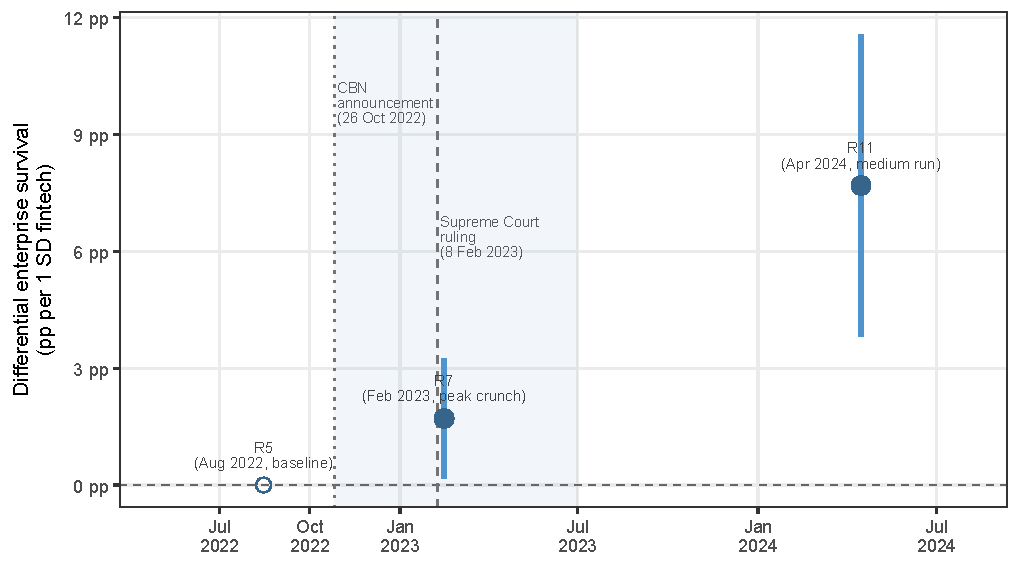
\includegraphics[width=0.94\textwidth]{figures/fig_eventstudy_firm.pdf}
\refstepcounter{figure}\label{fig:eventstudy_firm}
\floatfoot{%
  \textit{Notes:} Round-specific DiD coefficients from
  equation~\eqref{eq:firm}, plotting the differential enterprise survival
  probability (in percentage points) per one standard deviation of
  pre-shock fintech adoption ($\textit{Fintech}_s$).
  Round~5 (August 2022, pre-shock baseline) is the reference category
  (open circle, coefficient $= 0$ by construction).
  Solid circles are estimated coefficients; vertical bars are 95\%
  confidence intervals based on standard errors clustered at the
  state level. Shading marks the naira crunch window (CBN announcement
  to approximate cash normalisation). Dotted and dashed vertical lines
  mark the CBN announcement (26~October 2022) and Supreme Court ruling
  (8~February 2023) respectively. The \NLPS{} enterprise module was
  fielded only in Rounds~5, 7, and~11; there are no pre-shock
  enterprise observations.
}
\end{figure}

Table~\ref{tab:firm_did} presents estimates of equation~\eqref{eq:firm} for
three outcomes: an indicator for enterprise activity during the survey week
(columns 1--2), log weekly sales (columns 3--4), and the number of enterprise
workers (column 5). Odd columns omit sector and household controls; even
columns include them.

\begin{table}[H]
\caption{Firm-Level Effects of the Naira Crunch}
\label{tab:firm_did}

\begingroup
\centering
\begin{tabular}{lccccc}
   \tabularnewline \midrule \midrule
    & \multicolumn{2}{c}{Active} & \multicolumn{2}{c}{Log sales} & Workers \\ 
   Dependent Variables: & \multicolumn{2}{c}{active} & \multicolumn{2}{c}{ln\_sales} & n\_workers\\
   Model:                             & (1)            & (2)            & (3)            & (4)            & (5)\\  
   \midrule
   \emph{Variables}\\
   Fintech $\times$ R7 (peak crunch)  & 0.0171$^{**}$  & 0.0171$^{**}$  & 0.0184         & 0.0184         & 0.2940$^{***}$\\   
                                      & (0.0076)       & (0.0076)       & (0.0847)       & (0.0847)       & (0.0550)\\   
   Fintech $\times$ R11 (medium run)  & 0.0769$^{***}$ & 0.0769$^{***}$ & 0.3149$^{***}$ & 0.3149$^{***}$ &   \\   
                                      & (0.0192)       & (0.0192)       & (0.0925)       & (0.0925)       &   \\   
   Enterprise FE                      & \checkmark     & \checkmark     & \checkmark     & \checkmark     & \checkmark\\   
   Round FE                           & \checkmark     & \checkmark     & \checkmark     & \checkmark     & \checkmark\\   
   Rural control                      & No             & Yes            & No             & Yes            & No\\  
   \midrule
   \emph{Fixed-effects}\\
   hh\_f                              & Yes            & Yes            & Yes            & Yes            & Yes\\  
   round                              & Yes            & Yes            & Yes            & Yes            & Yes\\  
   \midrule
   \emph{Fit statistics}\\
   Observations                       & 5,269          & 5,269          & 3,482          & 3,482          & 3,084\\  
   R$^2$                              & 0.68987        & 0.68987        & 0.42580        & 0.42580        & 0.51830\\  
   Within R$^2$                       & 0.01309        & 0.01309        & 0.00530        & 0.00530        & 0.03387\\  
   \midrule \midrule
   \multicolumn{6}{l}{\emph{Clustered (state\_f) standard-errors in parentheses}}\\
   \multicolumn{6}{l}{\emph{Signif. Codes: ***: 0.01, **: 0.05, *: 0.1}}\\
\end{tabular}
 
\par \raggedright 
Sample: non-farm household enterprises active in NLPS Round 5 (August 2022 pre-shock baseline). Round 5 is the omitted baseline. Fintech is the standardised state-level digital payment index from NLPS Round 6 (October 2022). Workers only available for R5 and R7. Standard errors clustered at the state level. Inference robustness: see Appendix Table~\ref{atab:inference_robustness}.
\par\endgroup



\end{table}

Table~\ref{tab:firm_did} reports the main firm-level results. Enterprises in states one standard
deviation above the pre-shock fintech mean were 1.7 percentage points more
likely to remain in operation at the February 2023 peak crunch
($\hat\delta_{R7} = 0.017$, $p = 0.030$). Appendix
Table~\ref{atab:inference_robustness} reports inference under pairs bootstrap
and randomisation inference; under randomisation inference the R7 survival
effect is significant at the 10\% level ($p_{\text{RI}} = 0.085$), while the
R11 survival and R7 employment results remain significant at the 1\% level
under all inference methods. The R7 result should therefore be read as
suggestive support of the peak-crunch insulation channel, with R11
survival and employment providing the bedrock evidence. By April 2024 (Round~11, 14~months post-peak), 
the survival advantage has \emph{widened} to 7.7 percentage points ($p < 0.001$), indicating that the
initial resilience compounded into a durable medium-run advantage rather than
dissipating.

Employment results shows that enterprises in high-fintech states
had 0.29 more workers at peak crunch per standard deviation of fintech
($p < 0.001$). Log weekly sales at peak crunch (R7) are positive (0.018) but
statistically indistinguishable from zero ($p = 0.83$). A plausible
explanation is positive survivor selection in low-fintech states such that enterprises
that \emph{remained open} in low-fintech states at R7 were positively selected
on productivity, only the most efficient firms survived, compressing the
observable sales differential among survivors. Appendix
Table~\ref{atab:sales_decomp} provides formal evidence for this mechanism, where
pre-shock (R5) log sales are 0.162 log points higher among R7-survivors than
exiters in the low-fintech tercile, but 0.475 points \emph{lower} among
survivors versus exiters in the high-fintech tercile, confirming that
low-fintech survivors constitute a positively selected sub-sample.

On the other hand, the medium-run log-sales coefficient at R11 is large and
significant, $\hat\delta_{R11} = 0.315$ ($p < 0.001$), indicating
approximately 37\% higher weekly sales in high-fintech states fourteen months
after the peak. The R11 log-sales regression conditions on survival to
Round~11; that is, the comparison is restricted to enterprises that remained
active in both high- and low-fintech states. By April~2024, additional exit in
low-fintech states between R7 and R11 has depleted even the positively-selected
survivors identified at R7, leaving a residual sample that is thinner and
drawn from the lower tail of the low-fintech productivity distribution. The
widening sales gap at R11 therefore suggests the \emph{compounding} of two
forces: a genuine long-run divergence in productivity between enterprises that
maintained sales relationships and supplier networks through the crunch, and a
composition effect as continued exit in low-fintech states erodes the
survivor-selection buffer that suppressed the gap at R7. Both forces are indicative of a
persistent real cost of cash supply shocks in states with weak digital
infrastructure.

The medium-run survival gap at R11, 7.7 percentage points, is particularly noteworthy. 
The 16-percentage-point decline in enterprise activity from R5 to
R11 was not equally distributed as it was concentrated in low-fintech states
where the crunch proved a permanent exit shock for many small enterprises.

\subsection{Heterogeneity}
\label{sub:heterogeneity}

Table~\ref{tab:heterogeneity} presents two heterogeneity dimensions. Rural
versus urban location, and small versus large enterprises (split at the median
baseline worker count). The fintech insulation effect is concentrated in rural
enterprises (R7 coefficient of 0.026, $p = 0.015$) and small enterprises
(0.038, $p = 0.019$), while the urban and large-enterprise coefficients are
smaller and not statistically significant. This gradient is consistent with
the underlying mechanism that rural and small enterprises are more exclusively
dependent on physical cash for both receipts and payments, with fewer access
points to POS machines or formal banking buffers. Large urban enterprises
are better diversified across payment channels, reducing the marginal benefit
of state-level fintech infrastructure.

\begin{table}[H]
\caption{Heterogeneity by Location and Firm Size}
\label{tab:heterogeneity}

\begingroup
\centering
\begin{tabular}{lcccc}
   \tabularnewline \midrule \midrule
                                      & Rural          & Urban          & Small          & Large \\   
   Dependent Variable: & \multicolumn{4}{c}{active}\\
   Model:                             & (1)            & (2)            & (3)            & (4)\\  
   \midrule
   \emph{Variables}\\
   Fintech $\times$ R7 (peak crunch)  & 0.0263$^{**}$  & 0.0004         & 0.0379$^{**}$  & -0.0065\\   
                                      & (0.0103)       & (0.0134)       & (0.0154)       & (0.0099)\\   
   Fintech $\times$ R11 (medium run)  & 0.0771$^{***}$ & 0.0700$^{***}$ & 0.0750$^{***}$ & 0.0698$^{***}$\\   
                                      & (0.0212)       & (0.0188)       & (0.0209)       & (0.0245)\\   
   \midrule
   \emph{Fixed-effects}\\
   hh\_f                              & Yes            & Yes            & Yes            & Yes\\  
   round                              & Yes            & Yes            & Yes            & Yes\\  
   \midrule
   \emph{Fit statistics}\\
   Observations                       & 3,765          & 1,504          & 2,497          & 2,772\\  
   R$^2$                              & 0.67312        & 0.73562        & 0.67448        & 0.70521\\  
   Within R$^2$                       & 0.01137        & 0.01629        & 0.01201        & 0.01309\\  
   \midrule \midrule
   \multicolumn{5}{l}{\emph{Clustered (state\_f) standard-errors in parentheses}}\\
   \multicolumn{5}{l}{\emph{Signif. Codes: ***: 0.01, **: 0.05, *: 0.1}}\\
\end{tabular}
 
\par \raggedright 
Dependent variable: enterprise active (binary). Split-sample estimates. Small = below-median workers at R5 baseline. Standard errors clustered at state level.
\par\endgroup



\end{table}

%% Section 7: Long-Run Effects

\section{Longer-Run Effects}
\label{sec:longrun}

\subsection{Persistence in the NLPS: Round 11 (April 2024)}

The medium-run estimates in Tables~\ref{tab:firm_did}
and~\ref{tab:heterogeneity} show a 7.7-percentage-point enterprise survival
gap 14~months after the peak crunch, together with the 0.315 log-point sales
advantage reconciled in Section~\ref{sub:nlps_results}. This section examines
the compositional dimensions of this persistence using additional
household-level outcomes from Round~11.

Two mechanisms could sustain persistent divergence. First, enterprises that
closed or contracted during the crunch may have lost market relationships,
supplier networks, or key workers that are costly to rebuild, a \emph{scarring}
effect on firm-level human and social capital. Second, the crunch may have
accelerated a permanent reallocation of economic activity from cash-intensive
markets toward digitally-enabled channels, raising the long-run returns to
digital adoption and widening the productivity gap between high- and
low-fintech states.

Evidence from the household wage-employment panel (R5 to R11, column~1 of
Appendix Table~\ref{tab:additional_outcomes}) is informative about which
mechanism dominates. High-fintech states exhibit \emph{larger declines} in
formal wage employment at R11, with a coefficient of $-0.042$ ($p = 0.006$).
At first, this appears to contradict the enterprise survival and
employment results. The explanation lies in composition such that in high-fintech states,
surviving enterprises absorbed displaced wage workers into own-account
enterprise employment during the crunch. By R11, a higher share of the working
population in high-fintech states is engaged in enterprise self-employment
(consistent with the survival advantage shown in Table~\ref{tab:firm_did})
rather than formal wage work, a shift that shows up as a \emph{decline} in
the wage-employment indicator. In low-fintech states, enterprise exit was more
widespread, leaving fewer self-employment opportunities and pushing displaced
workers into inactivity rather than enterprise formation. This reallocation
pattern is more consistent with the \emph{reallocation} mechanism than pure
scarring. The crunch appears to have permanently redirected economic activity
toward enterprise self-employment in states with adequate digital
infrastructure, while low-fintech states simply contracted.

\subsection{Cross-Wave Evidence from the WBES (2014 vs. 2025)}
\label{sub:wbes_longrun}

The World Bank Enterprise Survey was fielded in Nigeria in 2014 (pre-shock)
and again in 2025 (approximately two years post-peak), providing a
cross-section comparison of formal-sector firm characteristics.
Table~\ref{tab:wbes_crosswave} reports zone-level means of the
finance-exclusion cash-dependence index in each wave, the change, and
the corresponding change in power-outage incidence.

\begin{table}[H]
\begin{threeparttable}
\caption{WBES Cross-Wave: Cash Dependence and Power Outages, 2014 vs.\ 2025}
\label{tab:wbes_crosswave}
\small
\begin{tabular}{l
  S[table-format=1.3]
  S[table-format=1.3]
  S[table-format=-1.3]
  S[table-format=1.3]
  S[table-format=1.3]
  S[table-format=-1.3]}
\toprule
 & \multicolumn{3}{c}{Cash-dependence index}
 & \multicolumn{3}{c}{Pct.\ with power outages} \\
\cmidrule(lr){2-4}\cmidrule(lr){5-7}
{Zone} & {2014} & {2025} & {$\Delta$}
       & {2014} & {2025} & {$\Delta$} \\
\midrule
North Central & 0.397 & 0.506 & 0.109 & 0.807 & 0.799 & -0.008 \\
North East    & 0.360 & 0.541 & 0.181 & 0.832 & 0.672 & -0.160 \\
North West    & 0.445 & 0.489 & 0.044 & 0.689 & 0.600 & -0.089 \\
South East    & 0.435 & 0.561 & 0.126 & 0.893 & 0.787 & -0.106 \\
South South   & 0.475 & 0.457 & -0.018 & 0.880 & 0.853 & -0.027 \\
South West    & 0.435 & 0.458 & 0.023 & 0.755 & 0.871 & 0.116 \\
\midrule
All zones     & 0.425 & 0.502 & 0.077 & 0.810 & 0.764 & -0.046 \\
\bottomrule
\end{tabular}
\begin{tablenotes}
\footnotesize
\item \textit{Notes:} Cash-dependence index is the mean across three
  indicators: (i)~no checking or savings account (\texttt{k6}),
  (ii)~no active loan or line of credit (\texttt{k8}), and (iii)~rates
  access to finance as a major or very severe obstacle (\texttt{k30}).
  The index ranges from~0 (fully finance-integrated) to~1 (fully
  excluded). Zone-level means are computed from firm-level data.
  The 2014 sample covers 2,676 firms in 19 states (mapped to geopolitical
  zones); the 2025 sample covers 1,043 firms in all six zones.
  The two waves are treated as independent cross-sections.
  South West includes Lagos, the most financially developed state in
  Nigeria; the \emph{increase} in power outages there (column 6)
  likely reflects the worsening of the Lagos electricity grid
  independent of the cash crunch.
\end{tablenotes}
\end{threeparttable}
\end{table}

The cross-wave comparison provides descriptive evidence consistent with a
reinforcing exclusion dynamic. Cash dependence increased most in North
Central ($+0.109$) and North East ($+0.181$), the zones with the lowest
pre-shock fintech adoption, suggesting firms without digital access during
the crunch had less incentive to invest in such infrastructure post-crunch,
perpetuating their exclusion. The South South ($-0.018$) and South West
($+0.023$) show minimal change, consistent with both zones' higher baseline
digital payment penetration insulating firms from the long-run footprint of
the crunch.

These patterns are descriptive and cannot be given a causal interpretation.
With only six geopolitical zones, no firm-level panel identifier across
waves, and potentially differential compositional change in the 2025 sample,
these comparisons motivate rather than confirm the persistence mechanism.
They are nonetheless consistent in direction with the \NLPS{} panel evidence
and with models of technology adoption under network externalities, where an
initial advantage in digital infrastructure compounds over time.

%% Section 8: Conclusion

\section{Conclusion}
\label{sec:conclusion}

This paper studies the real effects of Nigeria's 2022--23 naira crunch, an
abrupt, policy-induced reduction in the supply of physical currency, and
the role of digital financial infrastructure in moderating those effects.
The primary evidence comes from a firm-level panel, exploiting pre-shock
cross-state variation in digital payment adoption, measured eleven days before
the \CBN{} announcement, the studys shows large and persistent effects
on enterprise survival and employment. A 45-month pre-shock nighttime-light panel for all 774 Nigerian local
government areas validates the parallel-trends assumption as high- and
low-fintech states followed statistically identical \NTL{} trajectories before
the crunch, and the identifying assumption is robust to pre-trend violations
up to 20 times the observed magnitude.

First, enterprises in higher-fintech states were 1.7 percentage points
more likely to remain in operation at the February 2023 peak crunch, had
0.29 more workers, and the survival advantage widened to 7.7 percentage
points by April 2024. Effects are concentrated among rural and small
enterprises, the units most exclusively dependent on physical cash. 
Pairs bootstrap and randomisation-inference $p$-values confirm the R11 survival
and R7 employment results hold at the 1\% level under all inference methods;
the R7 survival effect is significant at the 10\% level under randomisation
inference and read as supportive evidence of peak-crunch insulation. 
Second, the 2025 \WBES{} cross-section
provides descriptive evidence of elevated cash dependence in low-fintech
zones, consistent with a reinforcing dynamic that the crunch appears to have
entrenched financial exclusion where digital infrastructure was thinnest.

To quantify the aggregate stakes and applying sampling weights to the Round~5
enterprise module yields approximately 20.5~million non-farm household
enterprises in Nigeria at the pre-shock baseline. Closing the fintech gap
between the 10th- and 90th-percentile state (a 1.85 standard-deviation
difference) would have reduced enterprise closures at peak crunch by
approximately 648,000 enterprises and preserved approximately 11~million
enterprise-worker positions during the most acute phase of the shortage.
By April 2024, the cumulative survival advantage translates to approximately
2.9~million fewer enterprise closures relative to a counterfactual of
homogeneous low-fintech adoption.

\paragraph{Policy implications.}
First, the results quantify a
macroeconomic stabilisation benefit of digital payment infrastructure that
is distinct from its better-documented microeconomic benefits for individual
households \citep{jack2014risk,suri2016mobile}. Digital payment systems do
not merely redistribute welfare within an economy; they reduce the aggregate
cost of a cash supply shock to the economy as a whole. This stabilisation
benefit should enter the \CBN's cost--benefit calculus when designing currency
operations, implementing withdrawal limits, or accelerating the rollout of
the e-Naira central bank digital currency.

Second, the results suggest that the sequencing of currency policy matters.
The naira crunch appears to have widened the digital--financial divide, as
firms in low-fintech zones entered a persistent cycle of exclusion. This
implies that currency redesigns or cash-withdrawal restrictions deployed
before digital payment infrastructure has reached a critical mass can have
lasting adverse effects on financial inclusion, the opposite of their stated
objective. Policy makers should ensure adequate digital payment coverage
before constraining cash supply.

\paragraph{Generalisability.}
While the estimates are identified from a single episode in Nigeria, the
mechanism, digital payments as a substitute transaction medium when cash is
scarce, is general. The satellite--survey methodology employed here
is directly transferable to other African economies or low-income settings, 
offering a way for empirical assessment in environments where macroeconomic data are limited, unavailable or lagged.

\paragraph{Limitations.}
First, the \NLPS{} enterprise panel tracks
household enterprises, which are likely more cash-intensive than the
formal-sector firms in the \WBES{}; the two samples are not directly
comparable. Second, the causal interpretation of the long-run \WBES{}
comparison requires the assumption that zone composition did not change
differentially across zones between 2014 and 2025, an assumption this study was unable to
verify from the public-release data.


% ── References ────────────────────────────────────────────────────────────────
\clearpage
\bibliography{references}

% ── Appendix ──────────────────────────────────────────────────────────────────
\clearpage
\begin{appendices}
%% Appendix

\section{Data Construction Details}
\label{asec:data_construction}

\subsection{VIIRS Nighttime Lights}
\label{asec:viirs_construction}

The monthly \VIIRS{} composites were extracted via Google Earth Engine
using the VNP46A3.001 product (NASA Black Marble Monthly). For each
of the 774 geopolitical units in the GeoBoundaries Nigeria ADM2
shapefile, the mean radiance of the \texttt{NearNadir\_Composite\_Snow\_Free}
layer was computed over all cloud-free pixels within the LGA polygon.
All regressions use the full panel; the NTL data serve as a pre-trend
validation tool rather than a primary outcome.

The LGA panel was merged to the GADM ADM1 (state) boundaries via
spatial centroid join: the centroid of each geoBoundaries polygon
was matched to its enclosing GADM state polygon, with a nearest-feature
fallback for coastal LGAs whose centroid falls offshore.

\subsection{Fintech Index Construction}
\label{asec:fintech_construction}

The composite fintech index is constructed from \NLPS{} Round~6
Section~5 (financial services module). For each household $h$ in
state $s$, binary indicators $d_{hj} \in \{0,1\}$ are constructed
for whether the household used service category $j \in \{3,5,6,7\}$
(mobile money, bank account, mobile/\textsc{ussd}, mobile app)
in the previous month. The household-level index is
$\textit{FintechIndex}_h = \frac{1}{4}\sum_{j} d_{hj}$, bounded in
$[0,1]$. The state-level index is the mean across households:
$\textit{Fintech}_s = \overline{\textit{FintechIndex}}_{h \in s}$.
In regressions it is standardised to mean~0, \textsc{sd}~1 across
states.

\subsection{WBES Finance-Exclusion Index}
\label{asec:wbes_construction}

The firm-level cash-dependence index used in Section~\ref{sub:wbes_longrun}
combines three binary indicators from the 2014 \WBES{}:
$b_1 = \mathbf{1}[\texttt{k6} = \text{No}]$ (no checking or savings account),
$b_2 = \mathbf{1}[\texttt{k8} = \text{No}]$ (no active loan or credit line),
and $b_3 = \mathbf{1}[\texttt{k30} \geq \text{Major obstacle}]$.
The firm-level index is $\textit{CashDep}_i = (b_1+b_2+b_3)/3$.
State-level aggregates are simple means across sampled firms.

\newpage

\section{Additional Tables and Figures}
\label{asec:additional}

% ── Fintech correlates ─────────────────────────────────────────────────────────
\begin{table}[H]\begin{threeparttable}
\caption{Pre-Shock Fintech Index: State-Level Correlates}
\label{atab:fintech_correlates}\small
\begin{tabular}{lc}\toprule
Variable & Corr.\ with Fintech index \\\midrule
Mean NTL 2019--2021 (log) & -0.19 \\
NTL growth 2019--2021 & 0.1 \\
WBES pct.\ unbanked (2014) & 0.34 \\
Log road dist.\ to hub & 0.13 \\
Terrain ruggedness (std.) & -0.51 \\
\bottomrule\end{tabular}
\begin{tablenotes}\footnotesize
\item \textit{Notes:} Pairwise Pearson correlations across 17 states. Fintech is moderately correlated with pre-2022 NTL level ($r=-0.19$) and essentially uncorrelated with pre-2022 NTL growth ($r=0.10$), supporting the parallel-trends assumption.
\end{tablenotes}\end{threeparttable}\end{table}


\clearpage

% ── Pre-trend sensitivity (NTL event study) ───────────────────────────────────
\begin{table}[H]
\begin{threeparttable}
\caption{Pre-Trend Sensitivity: Honest Confidence Intervals for the NTL Treatment Effect}
\label{atab:pretrend_sensitivity}
\small
\begin{tabular}{lllcc}
\toprule
$M$ & 95\% CI on $\hat{\beta}_{\text{peak}}$ & 95\% CI on $\hat{\beta}_{k=14}$ & Peak $>0$ & $k{=}14$ $>0$ \\
\midrule
0.0000 & [-0.0135, 0.0390] & [-0.0658, -0.0109] & No & No \\
0.0001 $\leftarrow$ obs.\ gradient & [-0.0139, 0.0394] & [-0.0671, -0.0096] & No & No \\
0.0001 $\leftarrow$ obs.\ gradient & [-0.0143, 0.0398] & [-0.0684, -0.0082] & No & No \\
0.0002 $\leftarrow$ obs.\ gradient & [-0.0147, 0.0402] & [-0.0698, -0.0069] & No & No \\
0.0003 & [-0.0151, 0.0406] & [-0.0711, -0.0056] & No & No \\
0.0003 & [-0.0155, 0.0410] & [-0.0724, -0.0043] & No & No \\
0.0004 & [-0.0160, 0.0415] & [-0.0742, -0.0025] & No & No \\
\bottomrule
\end{tabular}
\begin{tablenotes}
\footnotesize
\item \textit{Notes:} Sensitivity analysis in the spirit of \citet{rambachandran2023pretrends}. $M$ is the maximum allowed per-period (monthly) deviation from parallel trends. For each $M$, the honest confidence interval is computed as $[\hat{\beta}_k - 1.96 \hat{\sigma}_k - M \cdot |k - k_{\text{ref}}|,\;\hat{\beta}_k + 1.96 \hat{\sigma}_k + M \cdot |k - k_{\text{ref}}|]$, where $k_{\text{ref}} = -6$ (August 2022, the omitted reference period). The observed pre-period gradient is $M_{\text{obs}} = 0.0001$. $M^* = -0.0023$ is the violation required to make the lower bound exactly zero at the peak crunch period. The ratio $M^*/M_{\text{obs}} = -21.64$ indicates the pre-trend gradient would need to be amplified by this factor to overturn the NTL result. The firm-level pre-trend is validated separately via the NTL pre-period window; household and enterprise fixed effects in the firm panel absorb all time-invariant heterogeneity, making the firm-level estimates more robust to this concern.
\end{tablenotes}
\end{threeparttable}
\end{table}


\begin{figure}[H]
\centering
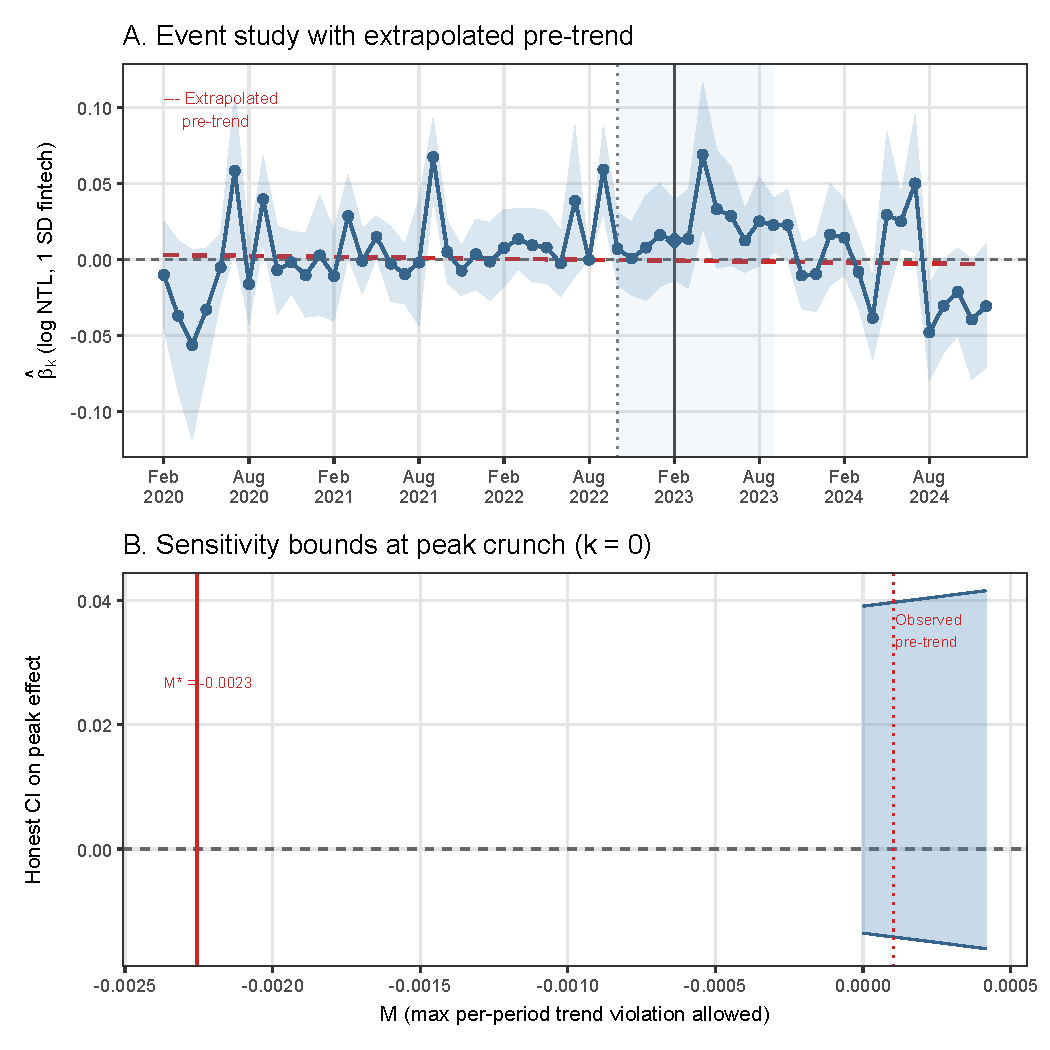
\includegraphics[width=\textwidth]{figures/fig_pretrend_sensitivity.pdf}
\caption{Pre-Trend Sensitivity Analysis}
\label{afig:pretrend_sensitivity}
\floatfoot{%
  \textit{Notes:} Panel A plots the \NTL{} event-study coefficients with the
  extrapolated pre-period trend line (dashed red). Panel B shows how the honest
  confidence interval on the peak-crunch coefficient evolves as the allowed
  per-period trend violation $M$ increases. The solid vertical line marks
  $M^* = 0.00226$, the violation required to make the lower bound touch zero.
  The dotted line marks the observed pre-period gradient $M_{\text{obs}} = 0.0001$.
  See Appendix~Table~\ref{atab:pretrend_sensitivity} for full details.
}
\end{figure}

\clearpage

% ── State trend robustness ────────────────────────────────────────────────────
\begin{figure}[H]
\centering
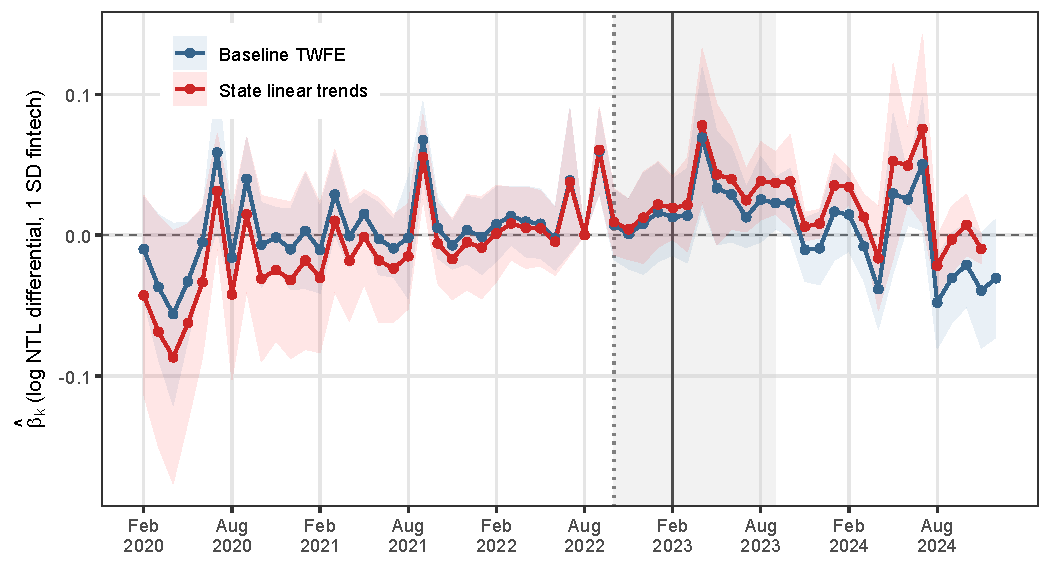
\includegraphics[width=\textwidth]{figures/fig_eventstudy_trend.pdf}
\caption{NTL Event Study: Baseline vs.\ State-Specific Linear Trend Robustness}
\label{afig:eventstudy_trend}
\floatfoot{%
  \textit{Notes:} Both lines plot round-by-round coefficients on
  $\textit{Fintech}_s \times \mathbf{1}[t=k]$ from a regression of
  $\ln(\NTL_{lt}+1)$ on state and month-year fixed effects, for baseline
  \textsc{twfe} (blue) and a specification that adds a state-specific linear
  time trend (red, dashed). The pre-period gradient is near zero in both
  specifications, validating the parallel-trends assumption. The
  trend-adjusted model shows attenuated post-announcement coefficients,
  reflecting the well-known sensitivity of state-trend specifications when
  the trend is estimated over a sample window that includes the shock period.
  Standard errors clustered at the state level.
}
\end{figure}

\clearpage

% ── Inference robustness ─────────────────────────────────────────────────────
\begin{table}[H]
\begin{threeparttable}
\caption{Firm-Level Inference Robustness: Pairs Bootstrap and Randomization Inference}
\label{atab:inference_robustness}
\small
\begin{tabular}{lcccccc}
\toprule
Outcome $\times$ Round & Coef. & Asy.\ SE & $p_{\text{asy}}$ & Boot.\ SE & $p_{\text{boot}}$ & $p_{\text{RI}}$ \\
\midrule
Enterprise active $\times$ R7 (peak crunch) & 0.0171 & 0.0076 & 0.030** & 0.0089 & 0.048** & 0.085* \\
Enterprise active $\times$ R11 (medium run) & 0.0769 & 0.0192 & 0.000*** & 0.0225 & 0.004*** & 0.000*** \\
Enterprise workers $\times$ R7 (peak crunch) & 0.2940 & 0.0550 & 0.000*** & 0.0659 & 0.002*** & 0.000*** \\
\bottomrule
\end{tabular}
\begin{tablenotes}
\footnotesize
\item \textit{Notes:} Each row reports inference for a focal hypothesis from the firm-level DiD specification (equation~\ref{eq:firm}). Coefficients are from Table~\ref{tab:firm_did}. Asy.\ SE: heteroskedasticity-robust SE clustered at the state level ($G=37$). Boot.\ SE: standard deviation of the coefficient across 999 pairs-bootstrap replications (states resampled with replacement). $p_{\text{boot}}$: fraction of centred bootstrap draws exceeding the observed absolute coefficient. $p_{\text{RI}}$: two-sided randomisation-inference $p$-value from 4999 permutations of the fintech index across states. $^{***}p<0.01$, $^{**}p<0.05$, $^{*}p<0.10$.
\end{tablenotes}
\end{threeparttable}
\end{table}


\clearpage

% ── Baseline balance ─────────────────────────────────────────────────────────
\begin{table}[H]
\begin{threeparttable}
\caption{Baseline Balance: Fintech and Pre-Shock Enterprise Characteristics}
\label{atab:balance}
\small\begin{tabular}{lcccc}
\toprule
Baseline characteristic & Coef. & SE & $p$-value & $N$ \\
\midrule
Log weekly sales (R5) & -0.0317 & 0.0528 & 0.552 & 1842 \\
Enterprise workers (R5) & -0.0780 & 0.0299 & 0.013** & 1842 \\
Rural enterprise & 0.0374 & 0.0470 & 0.431 & 1842 \\
Small firm & 0.0734 & 0.0215 & 0.002*** & 1842 \\
\bottomrule
\end{tabular}
\begin{tablenotes}\footnotesize
\item \textit{Notes:} Cross-sectional OLS at Round 5 (Aug 2022) baseline. Dependent variable is the listed enterprise characteristic. Regressor is the standardised state-level fintech index ($\textit{Fintech}_s$) measured in NLPS Round 6 (October 2022, 11 days before the CBN announcement). No fixed effects; standard errors clustered at the state level. Log weekly sales and rural location are balanced across the fintech distribution. Enterprise workers and small-firm status show statistically significant associations: high-fintech states have fewer enterprise workers ($p = 0.013$) and a higher share of small firms ($p = 0.002$) at baseline. These imbalances are absorbed by enterprise fixed effects in the main specification (equation~\ref{eq:firm}), which identifies off within-enterprise changes across rounds rather than cross-sectional differences. The heterogeneity results in Section~\ref{sub:heterogeneity} explicitly examine whether effects differ by firm size.
\end{tablenotes}\end{threeparttable}\end{table}


% ── Attrition test ────────────────────────────────────────────────────────────
\begin{table}[H]
\begin{threeparttable}
\caption{Attrition Test: Pre-Baseline Household Dropout and Fintech}
\label{atab:attrition}
\small\begin{tabular}{lcc}
\toprule
 & Coef. on Fintech & $p$-value \\
\midrule
Dropped from R3 to R5 baseline & -0.0340 & 0.203 \\
\bottomrule
\end{tabular}
\begin{tablenotes}\footnotesize
\item \textit{Notes:} Dependent variable = 1 if a household present in NLPS Round 3 (approx.\ Aug 2021) is absent from the Round 5 (Aug 2022) active enterprise sample. Regressor is the standardised state fintech index. A coefficient close to zero confirms that pre-baseline attrition is uncorrelated with the treatment variable.
\end{tablenotes}\end{threeparttable}\end{table}


\clearpage

% ── Sales null decomposition ──────────────────────────────────────────────────
\begin{table}[H]
\begin{threeparttable}
\caption{Survivor Selection and the Sales Null: Pre-Shock Sales by Fintech Tercile}
\label{atab:sales_decomp}
\small\begin{tabular}{lcccc}
\toprule
Fintech group & Survived to R7 & Exited by R7 & Difference & $N$ (surv/exit) \\
\midrule
Low fintech & 10.806 & 10.645 & 0.162 & 519 / 115 \\
Mid fintech & 10.594 & 10.928 & -0.334 & 508 / 133 \\
High fintech & 10.556 & 11.031 & -0.475 & 487 / 80 \\
\midrule
Interaction coef.\ (survived $\times$ fintech): & \multicolumn{3}{c}{-0.1699} & \\
$p$-value: & \multicolumn{3}{c}{0.131} & \\
\bottomrule
\end{tabular}
\begin{tablenotes}\footnotesize
\item \textit{Notes:} Mean log weekly sales at Round 5 (Aug 2022 pre-shock baseline) for enterprises that survived to R7 vs.\ those that had exited, by fintech tercile. If the log-sales null result at R7 reflects positive survivor selection in low-fintech states, the survival premium (survived minus exited) should be \emph{larger} in the Low fintech group. The interaction coefficient from OLS of R5 sales on survival status interacted with the continuous fintech index tests this formally; a negative coefficient would confirm stronger positive selection in low-fintech states. Standard errors clustered at the state level.
\end{tablenotes}\end{threeparttable}\end{table}


\clearpage

% ── Additional household outcomes ─────────────────────────────────────────────
\begin{table}[H]
\caption{Additional Household Outcomes: Wage Employment and Food Insecurity at Peak}
\label{tab:additional_outcomes}

\begingroup
\centering
\begin{tabular}{lccccc}
   \tabularnewline \midrule \midrule
    & Employed & \multicolumn{2}{c}{Food insecure} & Food worry & Food runout \\ 
   Dependent Variables: & employed & \multicolumn{2}{c}{food\_insecure} & food\_worry & food\_runout\\
   Model:                             & (1)             & (2)         & (3)         & (4)           & (5)\\  
   \midrule
   \emph{Variables}\\
   Fintech $\times$ R11 (medium run)  & -0.0423$^{***}$ &             &             &               &   \\   
                                      & (0.0145)        &             &             &               &   \\   
   Fintech index (std.)               &                 & -0.0083     & -0.0111     & -0.0308$^{*}$ & -0.0164\\   
                                      &                 & (0.0143)    & (0.0152)    & (0.0159)      & (0.0152)\\   
   Sample                             & Panel R5--R11   & R7 peak     & R7 peak     & R7 peak       & R7 peak\\  
   Household FE                       & \checkmark      & ---         & ---         & ---           & ---\\  
   Zone FE                            & ---             & \checkmark  & \checkmark  & \checkmark    & \checkmark\\   
   Round FE                           & \checkmark      & ---         & ---         & ---           & ---\\  
   Rural ctrl.                        & No              & No          & Yes         & Yes           & Yes\\  
   \midrule
   \emph{Fixed-effects}\\
   hh\_f                              & Yes             &             &             &               & \\  
   round                              & Yes             &             &             &               & \\  
   zone\_f                            &                 & Yes         & Yes         & Yes           & Yes\\  
   \midrule
   \emph{Fit statistics}\\
   Observations                       & 4,658           & 1,138       & 1,138       & 1,138         & 1,138\\  
   R$^2$                              & 0.63024         & 0.01475     & 0.01611     & 0.01833       & 0.02050\\  
   Within R$^2$                       & 0.00717         & 0.00015     & 0.00154     & 0.00328       & 0.00258\\  
   \midrule \midrule
   \multicolumn{6}{l}{\emph{Clustered (state\_f) standard-errors in parentheses}}\\
   \multicolumn{6}{l}{\emph{Signif. Codes: ***: 0.01, **: 0.05, *: 0.1}}\\
\end{tabular}
 
\par \raggedright 
Col (1): household wage-employment DiD (R5 Aug 2022 to R11 Apr 2024) with household FE. The negative coefficient indicates high-fintech states saw larger declines in formal wage employment, consistent with a composition shift toward self-employment in surviving enterprises (documented in Table~\ref{tab:firm_did}). Cols (2)--(5): food insecurity cross-section at R7 (peak crunch, Feb 2023). Treatment is state-level fintech index; zone FE (6 zones) absorb broad regional differences; state FE cannot be included as they are collinear with state-level treatment. Food insecure = 1 if household worried about or ran out of food in past month (FIES items). Cross-sections are descriptive; no household pre-period baseline is available. Standard errors clustered at the state level.
\par\endgroup



\end{table}

\clearpage

% ── IV first stage and leapfrog ───────────────────────────────────────────────
\begin{table}[H]
\caption{IV First Stage: Road Distance and Terrain Ruggedness}
\label{atab:iv_firststage}

\begingroup
\centering
\begin{tabular}{lcc}
   \tabularnewline \midrule \midrule
                                & (1)      & (2) \\   
   Dependent Variable: & \multicolumn{2}{c}{fintech\_std}\\
   Model:                       & (1)      & (2)\\  
   \midrule
   \emph{Variables}\\
   Constant                     & -0.9895  & -0.5092\\   
                                & (1.009)  & (1.014)\\   
   Log road dist.\ to hub (km)  & 0.2016   & 0.0960\\   
                                & (0.2027) & (0.2052)\\   
   Terrain ruggedness (std.)    &          & 0.4295$^{*}$\\   
                                &          & (0.2390)\\   
   \midrule
   \emph{Fit statistics}\\
   Observations                 & 37       & 37\\  
   R$^2$                        & 0.02749  & 0.11183\\  
   Adjusted R$^2$               & -0.00029 & 0.05958\\  
   \midrule \midrule
   \multicolumn{3}{l}{\emph{IID standard-errors in parentheses}}\\
   \multicolumn{3}{l}{\emph{Signif. Codes: ***: 0.01, **: 0.05, *: 0.1}}\\
\end{tabular}
 
\par \raggedright 
Cross-sectional OLS. Dependent variable: standardised fintech index (state level, NLPS Round 6). Road distance is the log km from each state centroid to the nearest qualifying financial hub. TRI is the mean terrain ruggedness index. Both instruments fail the relevance condition ($F<10$) and exhibit the wrong sign (states farther from hubs have higher fintech, reflecting the leapfrog dynamic documented in Appendix Table~\ref{atab:leapfrog}). Heteroskedasticity-robust standard errors.
\par\endgroup



\end{table}

\clearpage

\begin{table}[H]
\begin{threeparttable}
\caption{The Leapfrog Dynamic: Financial Exclusion (2014) and Fintech Adoption (2022)}
\label{atab:leapfrog}
\small\begin{tabular}{lccc}
\toprule
Geopolitical zone & Unbanked (2014, \%) & Fintech index (2022, \%) & States ($N$) \\
\midrule
3 & 38.3 & 30.3 & 7 \\
1 & 32.2 & 30.1 & 7 \\
4 & 30.7 & 25.6 & 5 \\
5 & 30.6 & 24.6 & 6 \\
6 & 21.1 & 24.4 & 6 \\
2 & 19.4 & 31.3 & 6 \\
\midrule
Pearson $r$ & \multicolumn{3}{c}{0.126} \\
\bottomrule
\end{tabular}
\begin{tablenotes}\footnotesize
\item \textit{Notes:} Zone-level means. Unbanked (2014) is the share of WBES 2014 firms without a bank account (proxy for initial financial exclusion). Fintech index (2022) is the mean state-level digital payment penetration from NLPS Round 6 (October 2022). The weak, near-zero correlation ($r=0.13$) between 2014 exclusion and 2022 fintech adoption reflects the leapfrog dynamic: zones that were most financially excluded in 2014 had the strongest incentive to adopt mobile money between 2014 and 2022, invalidating road distance to financial hubs as an instrument for fintech adoption. This explains the wrong-sign first-stage coefficient in Appendix Table~\ref{atab:iv_firststage}.
\end{tablenotes}\end{threeparttable}\end{table}


\clearpage


\begingroup
\centering
\begin{tabular}{lcc}
   \tabularnewline \midrule \midrule
   Dependent Variable: & \multicolumn{2}{c}{fintech\_std}\\
   Model:                                    & (1)                     & (2)\\  
   \midrule
   \emph{Variables}\\
   Constant                                  & $-2.75\times 10^{-17}$  & -1.399\\   
                                             & (0.1661)                & (1.031)\\   
   R1 digital payment index (std., Aug 2021) & 0.1877                  & 0.2530\\   
                                             & (0.1684)                & (0.1729)\\   
   Log road dist.\ to hub                    &                         & 0.2850\\   
                                             &                         & (0.2075)\\   
   \midrule
   \emph{Fit statistics}\\
   Observations                              & 37                      & 37\\  
   R$^2$                                     & 0.03431                 & 0.08511\\  
   Adjusted R$^2$                            & 0.00672                 & 0.03129\\  
   \midrule \midrule
   \multicolumn{3}{l}{\emph{IID standard-errors in parentheses}}\\
   \multicolumn{3}{l}{\emph{Signif. Codes: ***: 0.01, **: 0.05, *: 0.1}}\\
\end{tabular}
 
\par \raggedright 
Cross-sectional OLS. Dependent variable: standardised R6 fintech index (Oct 2022). Instrument: state-level share of households using any digital payment in NLPS Round 1 (August 2021, 14 months before the CBN announcement). This predetermines the fintech infrastructure readiness before the 2022-specific adoption dynamics. Heteroskedasticity-robust SEs.
\par\endgroup




\clearpage

% ── Alternative treatment index definitions ───────────────────────────────────
\begin{table}[H]
\caption{Robustness: Alternative Treatment Definitions}
\label{atab:alt_treatment}

\begingroup
\centering
\begin{tabular}{lcccc}
   \tabularnewline \midrule \midrule
                                  & Baseline (4-svc) & All 8 services & Payments only\\(mobile+USSD)   & Bank acct only \\   
   Dependent Variable: & \multicolumn{4}{c}{ln\_ntl\_mean}\\
   Model:                         & (1)              & (2)            & (3)                            & (4)\\  
   \midrule
   \emph{Variables}\\
   Fintech (4-svc) $\times$ Peak  & 0.0189           &                &                                &   \\   
                                  & (0.0154)         &                &                                &   \\   
   All-8 $\times$ Peak            &                  & 0.0315         &                                &   \\   
                                  &                  & (0.0248)       &                                &   \\   
   Payments-only $\times$ Peak    &                  &                & -0.0020                        &   \\   
                                  &                  &                & (0.0128)                       &   \\   
   Bank acct $\times$ Peak        &                  &                &                                & 0.0256\\   
                                  &                  &                &                                & (0.0153)\\   
   \midrule
   \emph{Fixed-effects}\\
   state                          & Yes              & Yes            & Yes                            & Yes\\  
   date\_fct                      & Yes              & Yes            & Yes                            & Yes\\  
   \midrule
   \emph{Fit statistics}\\
   Observations                   & 2,664            & 2,664          & 2,664                          & 2,664\\  
   R$^2$                          & 0.93148          & 0.93147        & 0.93083                        & 0.93126\\  
   Within R$^2$                   & 0.01016          & 0.01001        & 0.00086                        & 0.00705\\  
   \midrule \midrule
   \multicolumn{5}{l}{\emph{Clustered (state) standard-errors in parentheses}}\\
   \multicolumn{5}{l}{\emph{Signif. Codes: ***: 0.01, **: 0.05, *: 0.1}}\\
\end{tabular}
 
\par \raggedright 
Peak crunch period coefficient only. All specifications include state and month-year FEs. Column (3) uses only mobile money and USSD/mobile banking (the two categories most directly substitutable for cash during the crunch). Clustered SEs at the state level.
\par\endgroup



\end{table}

\clearpage

% Summary statistics appear in Table~\ref{tab:summary} of the main text (Section~\ref{sec:data}).

\end{appendices}

\end{document}
